Having assessed neural network performance across a range of ordinary differential equation problems,
we now turn to a more challenging class: partial differential equations (PDEs). In this section, 
we consider a single representative elliptic PDE posed on a two-dimensional domain:
\[
\begin{aligned}
    -\nabla^2 u(x, y) &= f(x, y), \quad \text{for } (x, y) \in \Omega := (0,1)^2, \\
    u(x, y) &= 0, \quad \text{for } (x, y) \in \partial \Omega,
\end{aligned}
\]
where the forcing function is given by
\[
f(x, y) = 13\pi^2 \sin(2\pi x)\sin(3\pi y).
\]
This problem admits an exact solution \( u(x, y) = \sin(2\pi x)\sin(3\pi y) \), which is smooth, bounded, 
and vanishes on the boundary of the domain.

Our goal is to assess the ability of neural networks to recover this solution from collocation data 
sampled over the interior and boundary of the domain. Based on prior results, we restrict our 
attention to the \(\tanh\) and Swish activation functions, as ReLU has been shown to perform poorly 
in earlier experiments. We follow a similar methodology to that used in the ODE setting: 
systematically varying depth and width of the network and evaluating performance using mean 
squared error over a dense evaluation grid. We sample 1000 points internally and 200 points 
from the boundary, all points being equidistantly spaced.

In addition to architectural comparisons, we also investigate the robustness of the best-performing 
networks to data scarcity. Specifically, we assess how the approximation quality degrades as 
the number of training (collocation) points is reduced, thereby evaluating the sample efficiency 
of neural networks in recovering PDE solutions from limited information.

\subsection{Architectural Performance on the Poisson Problem}

 Figure~\ref{fig:pde_comparison} shows the results of our architectural analysis. We observe
consistent trends across both activation functions: increasing network width generally 
leads to improved accuracy, while depth plays a subtler role. The best models for both $\tanh$ and 
Swish achieve high-quality approximations to the true solution, closely matching the ground truth 
throughout most of the domain. However, the absolute error plots reveal that the Swish-based network 
produces a slightly more accurate fit overall, particularly along the domain boundaries. While both 
models perform well in the central region, the $\tanh$ network exhibits noticeable deviations near the 
edges, whereas the Swish model only shows small discrepancies at the corners. This suggests that the 
Swish activation may offer improved boundary adherence in this context, potentially due to its smooth 
yet non-saturating properties.

\begin{figure}[htbp]
    \centering
    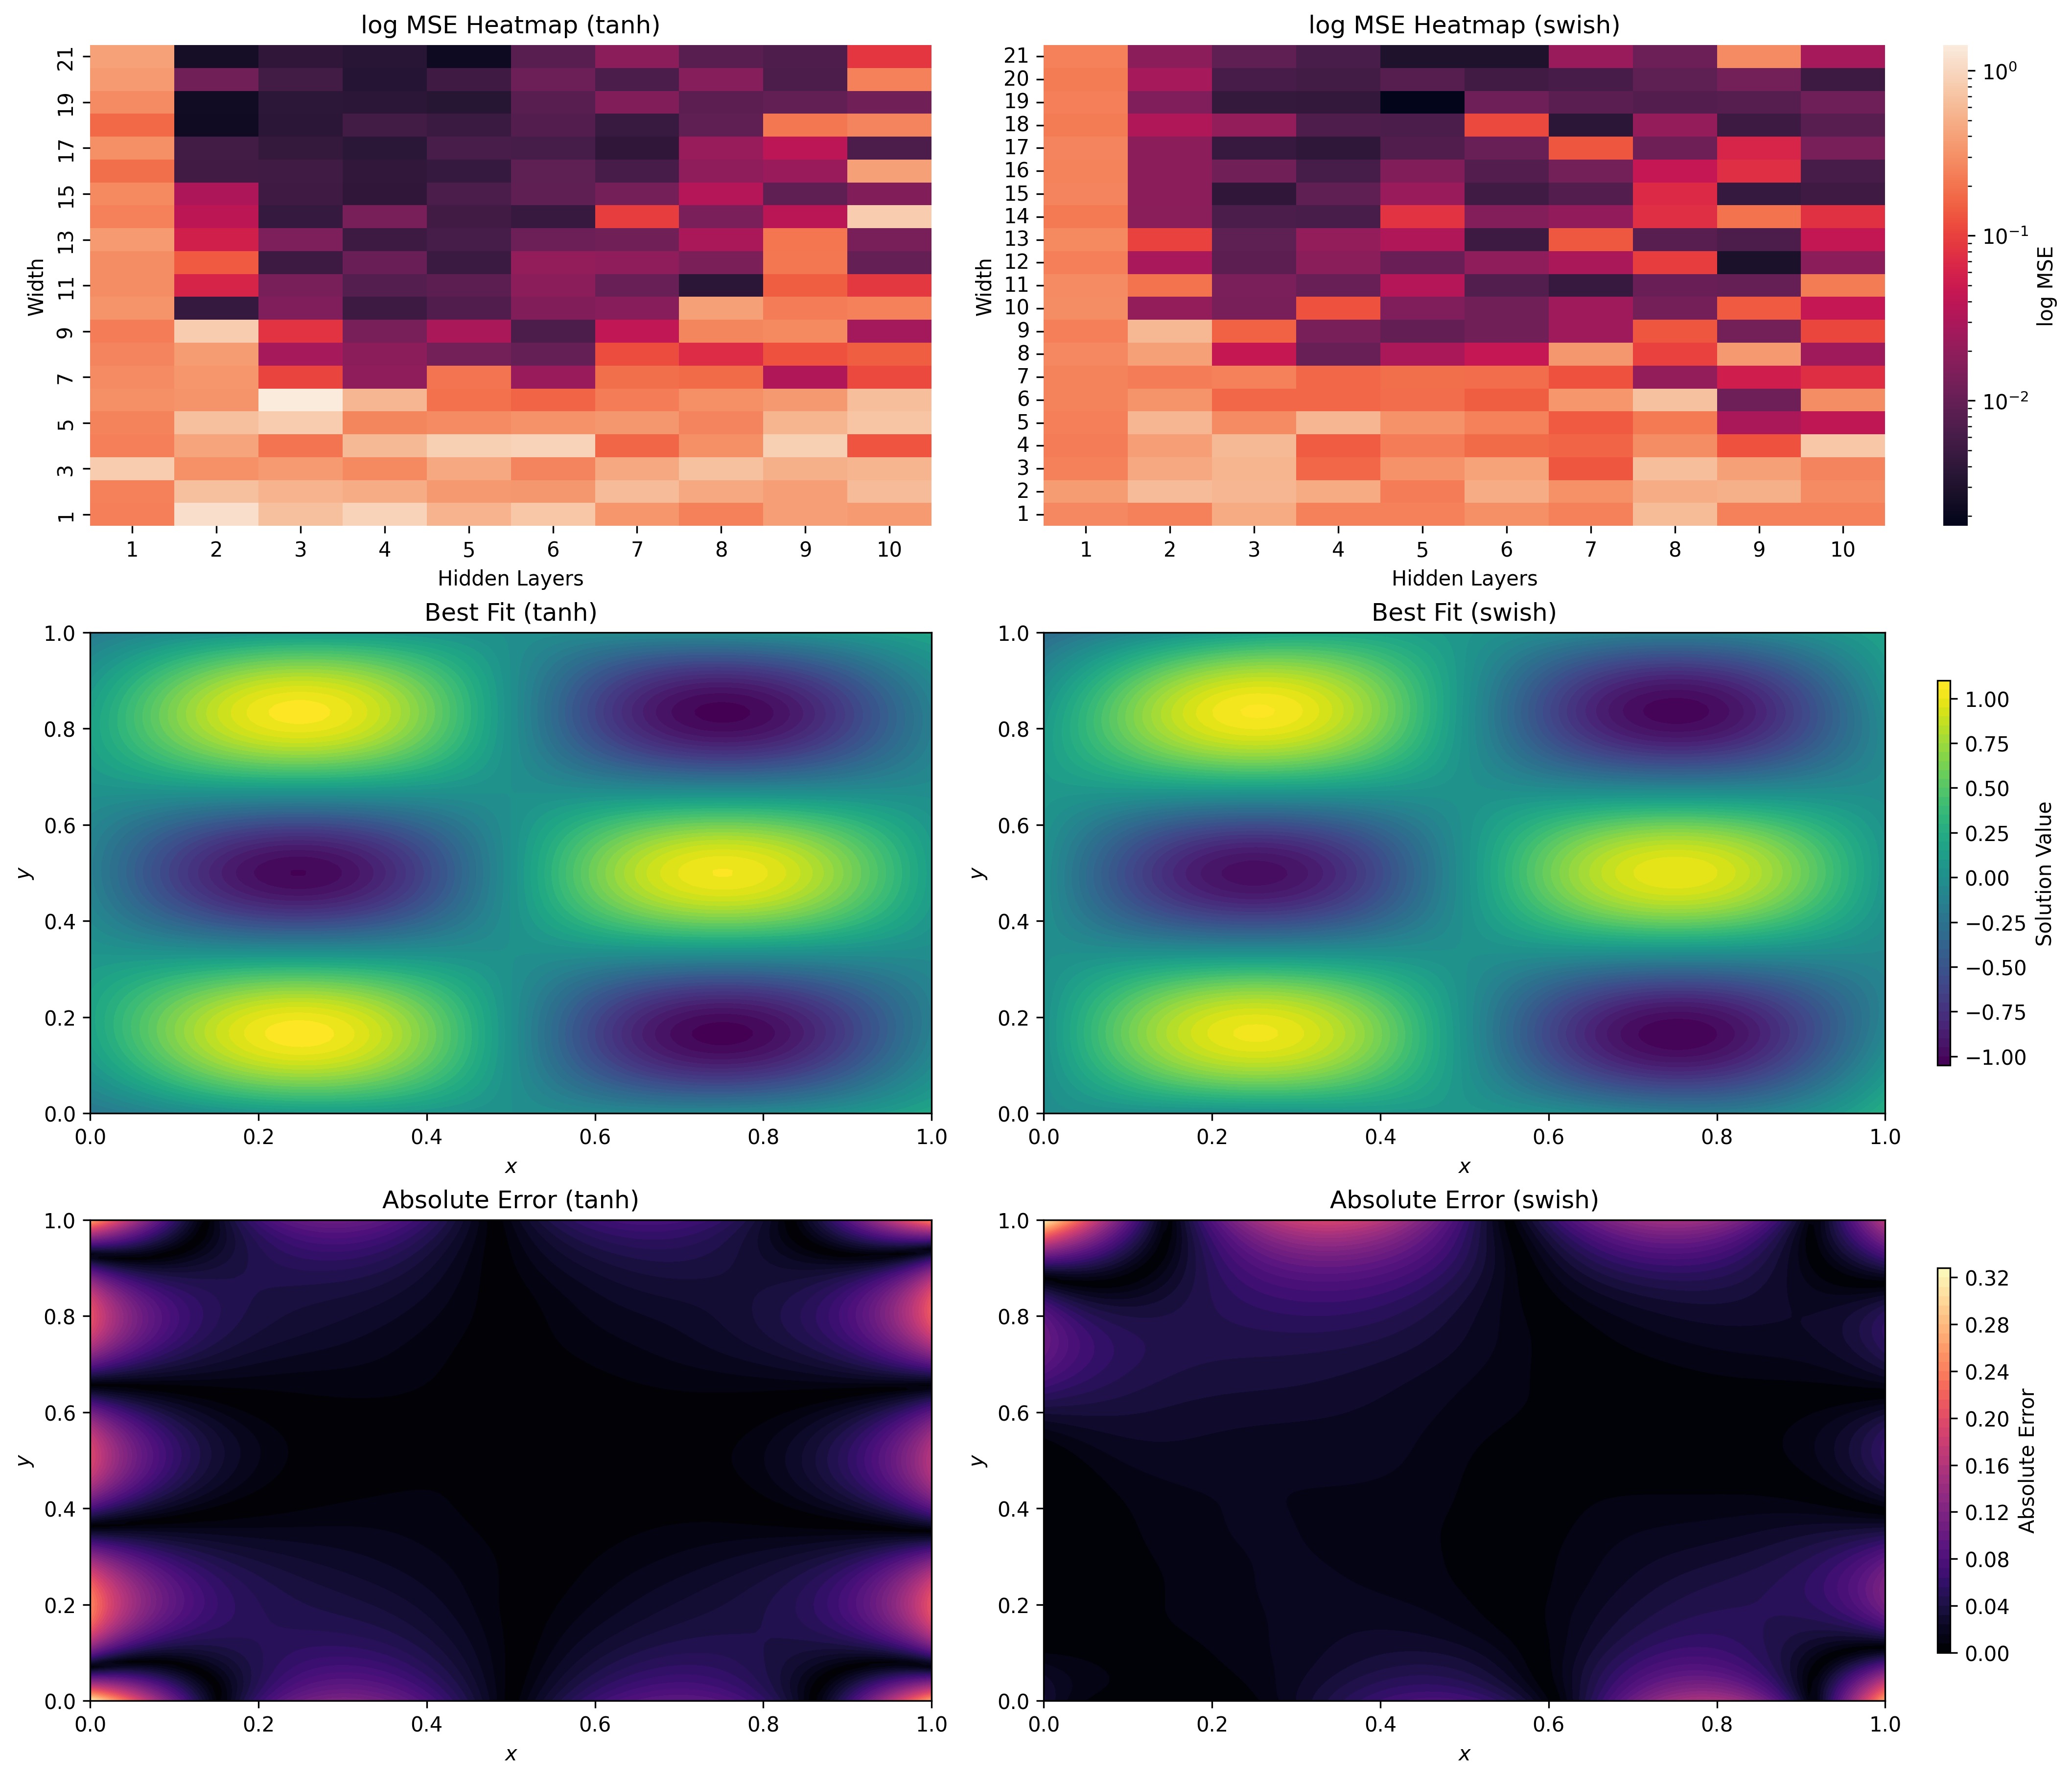
\includegraphics[width=0.9\textwidth]{graphics/pde_poisson_architecture_comparison.png}
    \caption{Comparison of neural network performance on the two-dimensional Poisson problem using the 
    $\tanh$ and Swish activation functions. Top row: log-scaled MSE heatmaps across architectural 
    configurations. Middle row: predicted solutions from the best-performing networks. Bottom row: 
    corresponding absolute error plots.}
    \label{fig:pde_comparison}
\end{figure}

We therefore elect to use the best-performing neural network from the above found, and now 
examine how this network performs as training points are reduced in the next section.

\subsection{Robustness to Reduced Training Data}

We now assess the sensitivity of neural network approximations to the number of training points, 
using the best-performing architecture from the preceding analysis. We vary the number of internal 
and boundary training points and illustrate the resulting accuracy in 
Figure~\ref{fig:training_point_comparison}.

\begin{figure}[t]
    \centering
    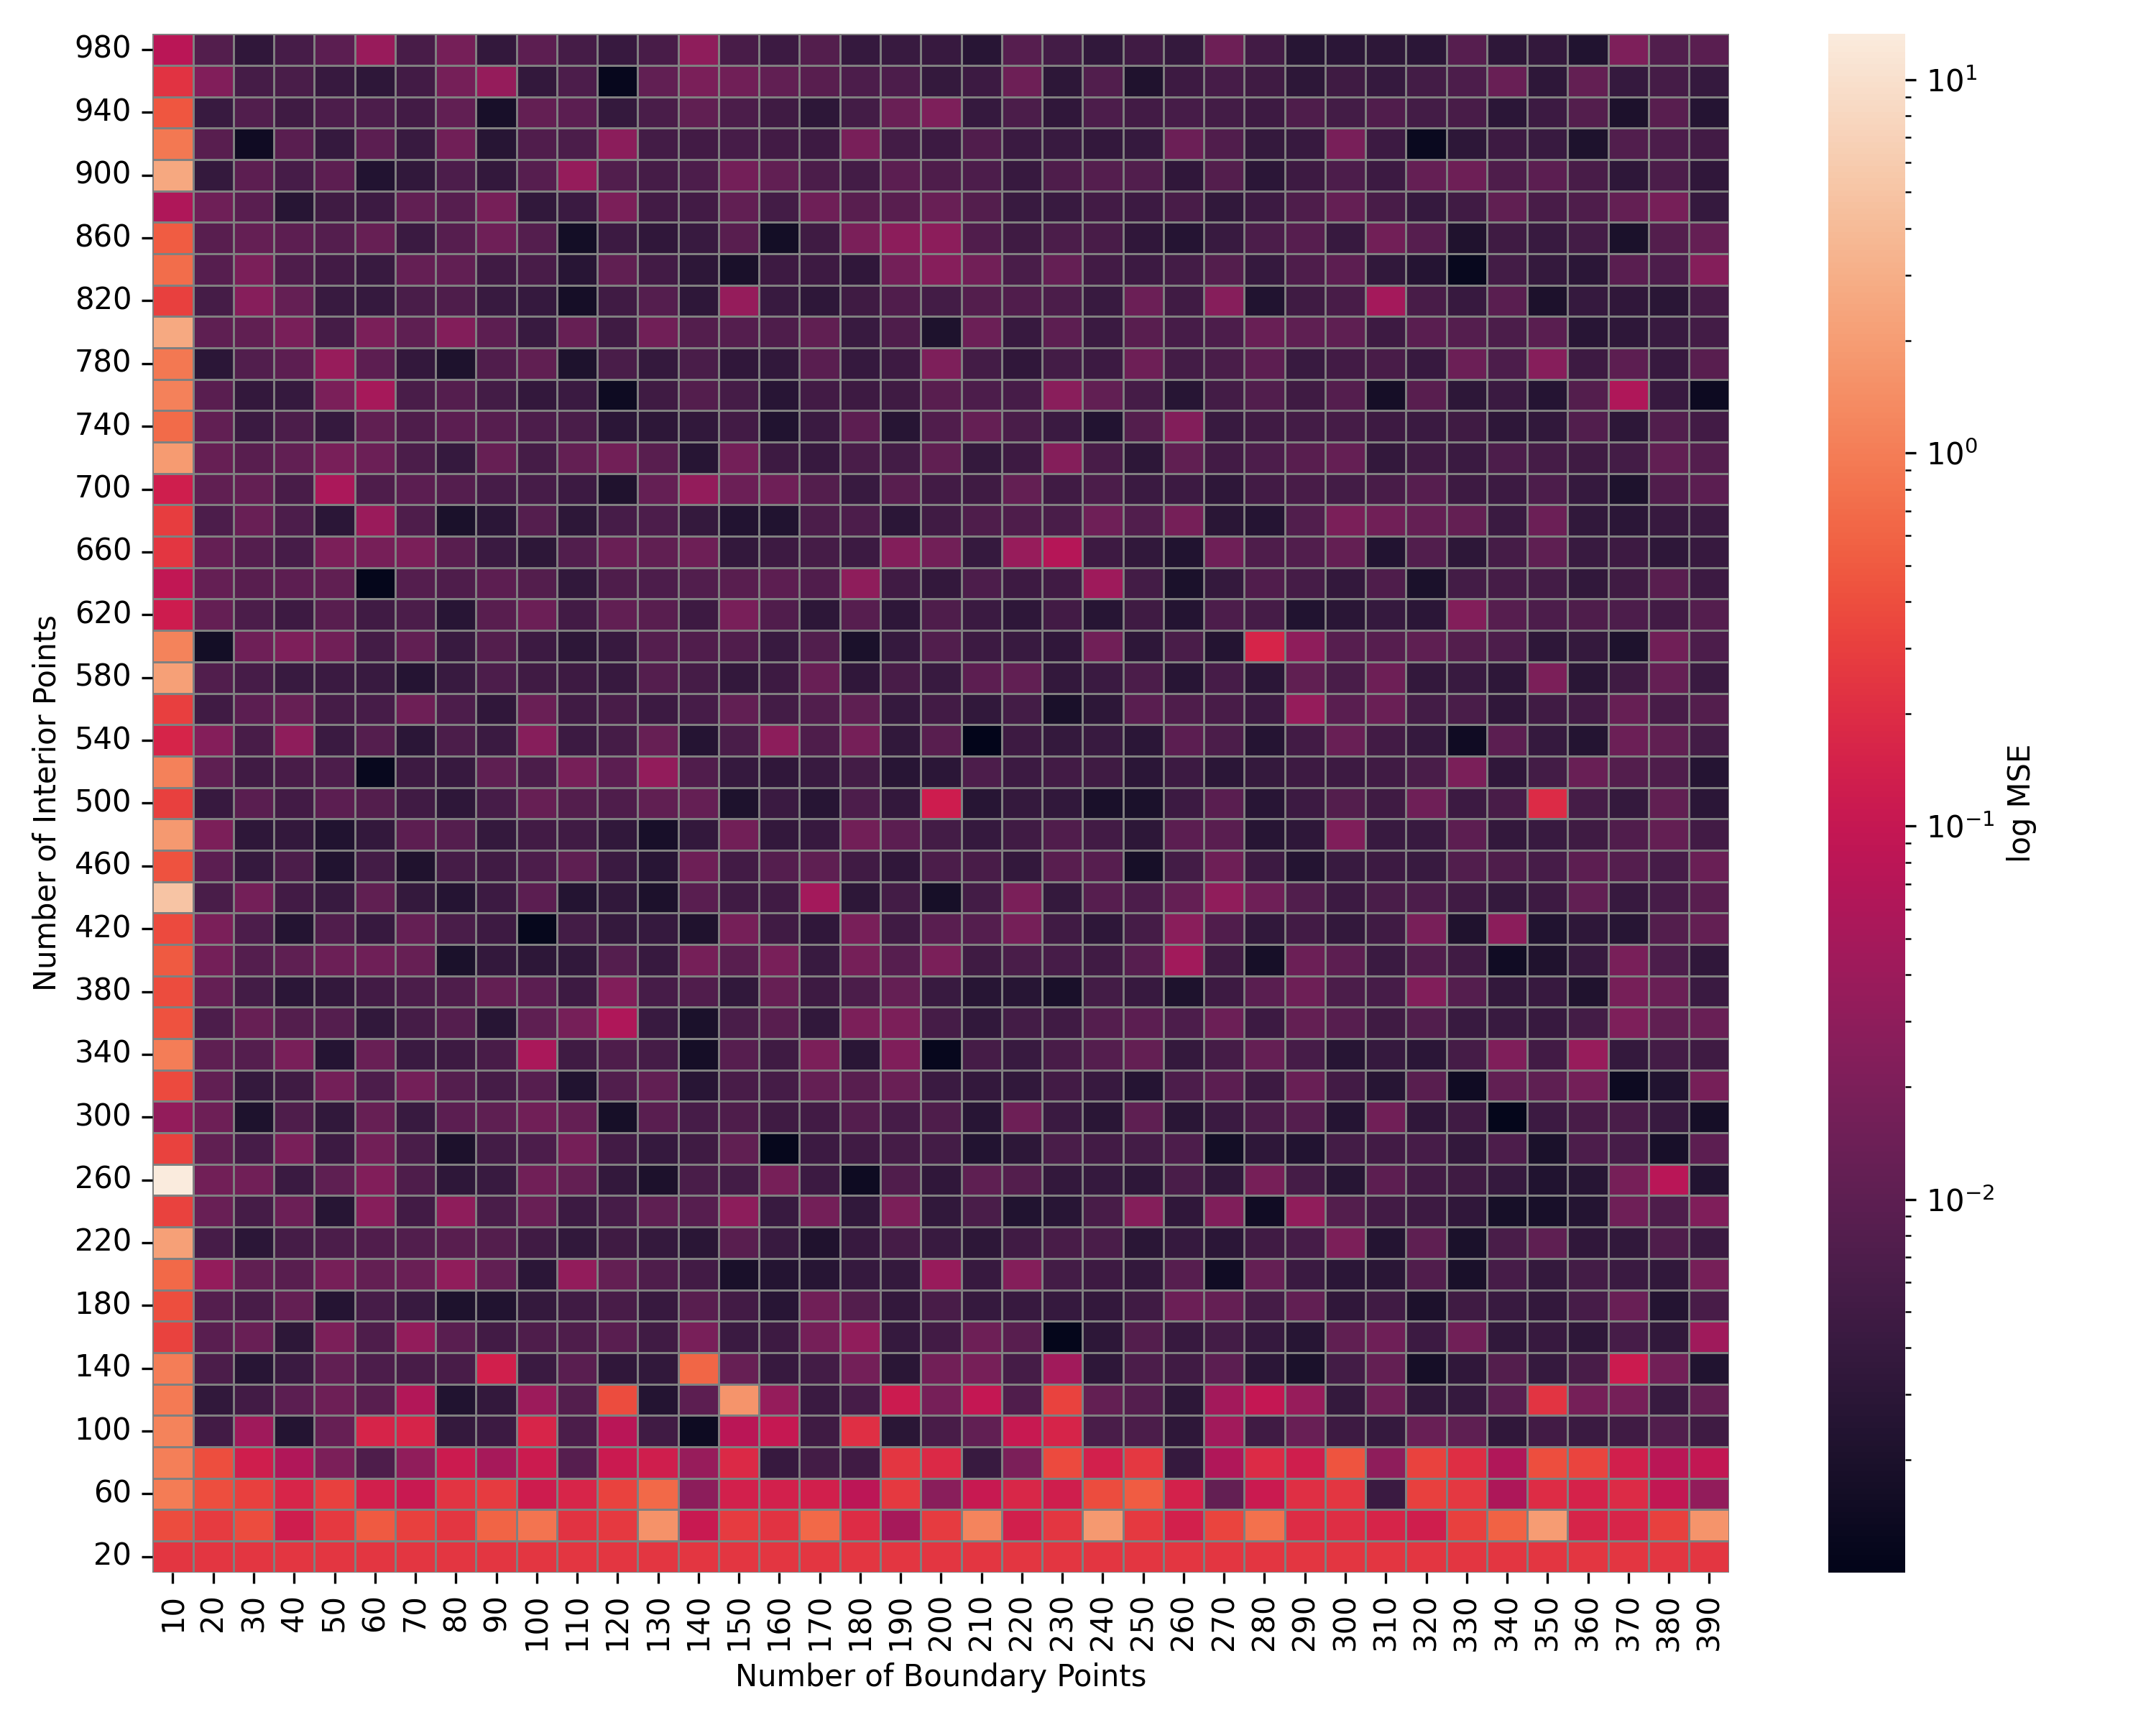
\includegraphics[width=0.75\textwidth]{graphics/pde_uniform_sampling_heatmap.png}
    \caption{Mean squared error heatmap showing how approximation accuracy varies with the number of internal and boundary training points.}
    \label{fig:training_point_comparison}
\end{figure}

The heatmap shows rapid convergence to high accuracy even with relatively sparse training points. 
Notably, performance improvements diminish significantly beyond approximately 100 internal points and
20 boundary points, indicating a clear threshold for obtaining an accurate solution. To better 
illustrate this threshold effect, Figure~\ref{fig:stacked_predictions} compares model predictions 
just below and at this threshold.

\begin{figure}[h]
    \centering
    \begin{subfigure}[t]{0.8\textwidth}
        \centering
        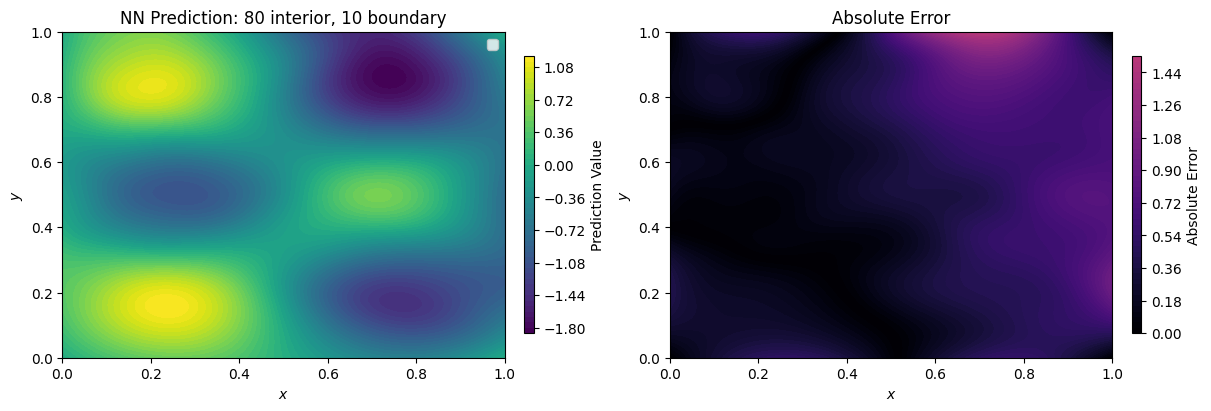
\includegraphics[width=\textwidth]{graphics/pde_points_80_10.png}
        \label{fig:prediction_80}
    \end{subfigure}
    
    \vspace{1em} 
    
    \begin{subfigure}[t]{0.8\textwidth}
        \centering
        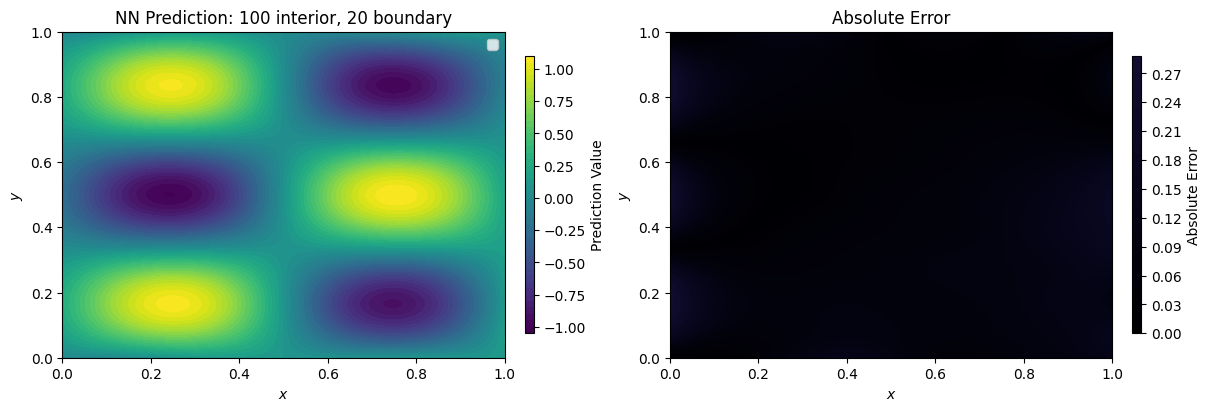
\includegraphics[width=\textwidth]{graphics/pde_points_100_20.png}
        \label{fig:prediction_100}
    \end{subfigure}
    \caption{Comparison of neural network predictions illustrating improved accuracy with moderate increases in training data.}
    \label{fig:stacked_predictions}
\end{figure}

Figure~\ref{fig:stacked_predictions} highlights how adding a modest number of training points 
substantially improves the accuracy and resolution of the neural network approximation. The 
prediction with 100 internal and 20 boundary points is notably sharper and exhibits significantly 
reduced error across the domain. The reported error in each case is computed as the mean squared 
error evaluated on 1000 equidistant points across the domain. These results confirm the robustness 
of neural network methods, achieving accurate PDE solutions with a relatively sparse distribution 
of training data.